% TELFOR 2026 — IEEE conference paper (A4, two-column)
% Overleaf: New Project -> Upload -> this file + refs.bib + figures/pareto.pdf
% Compile with pdfLaTeX. Page limit: 4.
%
% NAPOMENA: sav prozni tekst pišeš TI — mesta su označena sa:
%   % ================= TVOJ TEKST =================
% Tabele, figura i brojevi su izmereni podaci i spremni su.

\documentclass[conference,a4paper]{IEEEtran}
\usepackage[utf8]{inputenc}
\usepackage[T1]{fontenc}
\usepackage{graphicx}
\usepackage{booktabs}
\usepackage{amsmath}

% Copyright red za TELFOR — tačan string proveri u uputstvima na telfor.rs
% (obično oblika 979-8-3315-XXXX-X/26/\$31.00 ©2026 IEEE), pa odkomentariši:
% \IEEEoverridecommandlockouts
% \IEEEpubid{\makebox[\columnwidth]{XXX-X-XXXX-XXXX-X/26/\$31.00~\copyright2026 IEEE \hfill}}

\begin{document}

\title{Null Models and Sampling-Based Evaluation Expose the Real Value of
Reinforcement Learning for LLVM Pass Ordering}

\author{\IEEEauthorblockN{Dimitrije Pe\v{s}i\'c}
\IEEEauthorblockA{\textit{[Afilijacija — fakultet ili Independent Researcher]}\\
Belgrade, Serbia\\
dimitrije.pesicc@gmail.com}}

\maketitle

\begin{abstract}
% ================= TVOJ TEKST =================
% Tačke koje apstrakt mora da pokrije (vidi telfor_skeleton.md):
% RL za pass ordering se meri protiv -O3/-Oz sa argmax rollout-ima;
% mi uvodimo null-modele u kuriranom 36-pass prostoru + best-of-k
% sampling evaluaciju; 371+9 programa, 7 izvora; tri nalaza:
% (1) kurirani prostor + random pretraga tuče -Oz na svim real-code
% suite-ovima (granica: sintetički kod);
% (2) GNN politika kao sampler tuče fer null 24/24 (p=6e-8), dostiže
% greedy uz ~5x manje kompilacija;
% (3) RL sam ne trenira enkoder — distilacija Autophase featura ga
% otključava. Poruka: izbor merenja menja zaključke više nego izbor
% reprezentacije.
\end{abstract}

\begin{IEEEkeywords}
compiler optimization, LLVM, phase ordering, reinforcement learning,
graph neural networks, evaluation methodology
\end{IEEEkeywords}

\section{Introduction}
% ================= TVOJ TEKST =================
% (skica u telfor_skeleton.md, sekcija I)

\section{Related Work}
% ================= TVOJ TEKST =================
% Obavezno: AutoPhase \cite{autophase}, CompilerGym \cite{compilergym},
% ProGraML \cite{programl}, MLGO \cite{mlgo}, POSET-RL \cite{posetrl},
% Coreset \cite{coreset} (najbliži sused — diferencijacija!),
% Mammadli \cite{mammadli}, LLM Compiler \cite{llmcompiler}.

\section{Experimental Protocol}
% ================= TVOJ TEKST =================
% (skica u telfor_skeleton.md, sekcija III: CompilerGym llvm-ic-v0,
% 36-pass action space, PPO agenti, null-modeli, argmax vs sampling,
% suite-ovi, pretraining postupak)

\section{Results}

\subsection{Curated action space vs. -Oz}
% ================= TVOJ TEKST ================= (opis Tabele I)

\begin{table}[t]
\caption{Total IR instruction count per suite: real optimization levels
vs.\ best-of-50 random episodes in the curated 36-pass space.}
\label{tab:nulls}
\centering
\small
\begin{tabular}{lrrrrr}
\toprule
Suite ($n$) & O0 & -O3 & -Oz & Rnd-50 & $\Delta$Oz \\
\midrule
MiBench (40)   & 12{,}270  & 6{,}317  & 4{,}841  & \textbf{4{,}765}  & $+1.6\%$ \\
BLAS (50)      & 40{,}745  & 39{,}141 & 37{,}838 & \textbf{36{,}757} & $+2.9\%$ \\
cBench (9)     & 232{,}442 & 163{,}834& 115{,}987& \textbf{111{,}006}& $+4.3\%$ \\
CHStone (12)   & 19{,}857  & 14{,}182 & 9{,}834  & \textbf{9{,}097}  & $+7.5\%$ \\
POJ-104 (97)   & 21{,}099  & 11{,}083 & 8{,}334  & \textbf{7{,}622}  & $+8.5\%$ \\
NPB (122)      & 130{,}327 & 70{,}659 & 59{,}542 & \textbf{44{,}981} & $+24.5\%$ \\
\midrule
csmith (50)    & 352{,}963 & 82{,}950 & \textbf{57{,}625} & 60{,}626 & $-5.2\%$ \\
\bottomrule
\end{tabular}
\end{table}

\subsection{Argmax vs.\ sampling evaluation}
% ================= TVOJ TEKST ================= (opis Tabele II + statistika:
% GNN 24/24, sign test p=5.96e-8, Wilcoxon značajan na svih 7 suite-ova;
% AP 15/24, p=0.15 — identičan trening, drugačija reprezentacija)

\begin{table}[t]
\caption{Best-of-8 sampled rollouts (median seed) vs.\ the paired
best-of-8 random null and -Oz. Policies were trained on four small
cBench programs only.}
\label{tab:sampling}
\centering
\small
\begin{tabular}{lrrrr}
\toprule
Suite ($n$) & Null & -Oz & AP & GNN \\
\midrule
MiBench (40) & 4{,}828 & 4{,}841 & 4{,}783 & \textbf{4{,}782} \\
CHStone (12) & 9{,}241 & 9{,}834 & 9{,}133 & \textbf{9{,}120} \\
BLAS (50) & 37{,}099 & 37{,}838 & 36{,}998 & \textbf{36{,}847} \\
csmith (28) & 17{,}555 & 20{,}226 & 17{,}179 & \textbf{17{,}064} \\
NPB (120) & 40{,}301 & 53{,}085 & 40{,}822 & \textbf{39{,}909} \\
POJ-104 (97) & 7{,}853 & 8{,}334 & 7{,}917 & \textbf{7{,}730} \\
\bottomrule
\end{tabular}
\end{table}

\begin{figure}[t]
\centering
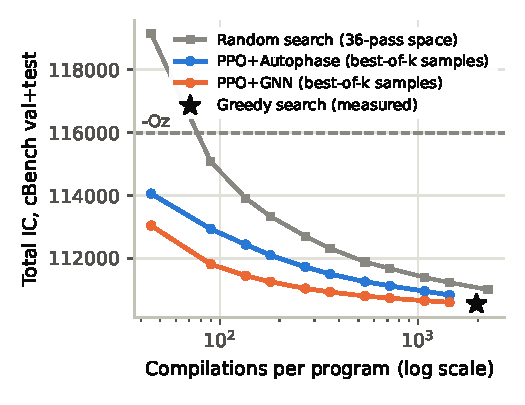
\includegraphics[width=\columnwidth]{figures/pareto.pdf}
\caption{Solution quality vs.\ compilation budget on cBench val+test.
Best-of-$k$ policy sampling against expected best-of-$k$ random search
and measured greedy search.
% NAPOMENA: posle k=32 sweep-a regeneriši figuru i ažuriraj opis.
}
\label{fig:pareto}
\end{figure}

\subsection{Encoder pretraining}
% ================= TVOJ TEKST ================= (opis Tabele III: 0/3 -> 2/2
% proboja platoa; popravlja argmax transfer ~9-12%; trade-off mod/distribucija)

\begin{table}[t]
\caption{Effect of Autophase-distillation pretraining on the GNN agent.}
\label{tab:pretrain}
\centering
\small
\begin{tabular}{lccc}
\toprule
GNN variant & val-small best & Full val & Full test \\
 & (per seed) & (argmax) & (argmax) \\
\midrule
From scratch & 689 / 689 / 689 & 64{,}550 & 69{,}180 \\
+ pretraining & \textbf{651 / 668} & \textbf{55{,}593} & \textbf{61{,}015} \\
\bottomrule
\end{tabular}
\end{table}

\subsection{Binary-level metrics}
% ================= TVOJ TEKST =================
% IZMERENO (results/binary_metrics/_aggregate.json, 371 programa):
% - .text (upareni skup, n=347): Oz 967,878 B; Rnd-bo8 866,989 B (+10.4%);
%   GNN-bo8 864,887 B (+10.6% manje od -Oz).
% - .text (pun skup, n=371, ukljucuje najvece csmith): Rnd-bo8 +4.0% vs Oz.
% - Primena sekvence (opt CLI, medijan po programu): nase sekvence
%   15.0-15.8 ms vs -Oz pipeline 19.5 ms (~20-25% brze) - sekvence rade
%   i van CompilerGym-a, kroz cist opt poziv.
% - IC->.text korelacija: r=0.78 (p=2.2e-6) na programima >=1000
%   instrukcija; ispod toga fiksni codegen overhead dominira.
% - footprint (text+data+bss) se ne menja - data/bss ne zavise od
%   redosleda prolaza (jedna recenica, posteno).

\section{Discussion and Limitations}
% ================= TVOJ TEKST =================
% (skica u telfor_skeleton.md, sekcija V — uključi .text anchor granicu,
% csmith granicu, CompilerGym 0.2.5 stack, preporuke za praksu evaluacije)

\section{Conclusion}
% ================= TVOJ TEKST =================

% \section*{Acknowledgment}
% The author thanks Prof.~[ime] for an early discussion of this work.

\bibliographystyle{IEEEtran}
\bibliography{refs}

\end{document}
